\subsection*{Aplicaciones del Algoritmo de Kruskal}

    Existen diversas aplicaciones del algoritmo en un escenario real mediante la industria.\\
    
    Los problemas más socorridos por este algoritmo son aquellos que tienen que ver con distancias y puntos fijos en un área geográfica. De esta forma el problema de la distribución de los cables a las tomas o estaciones fijas repartidas en la ciudad, a cargo empresas del sector de las telecomunicaciones y servicios eléctricos, se auxilian de este para identificar el cableado más corto y conecte a un número de nodos fijos, significa menores costos en muchos de los aspectos insfraestructurales.
    
    Así mismo, puede ser considerada una problemática similar la ruta que conecta estaciones perteneciente a algún servicio de transporte, tal como un Metro, Tren o similares. Este algoritmo les auxilia permientiendo no solo disminuir costos para la construcción, y mantenimiento, pero asegura la ruta que más rápidamente permite el transporte de los usuarios, significando un ahorro también en el tiempo.

\subsection*{Análisis a posteriori}
    Para obtener una gráfica descriptiva y que permitiera realizar un análisis mediante una aproximación de forma correcta, se decidió que se evaluarián, al menos, grafos con un número total de 10 nodos o aristas.
    
    Para la descripción de los grafos, se utilizaron archivos donde cada fila corresponde a la descripción de un nodo. La sintaxis para la descripción del nodo inicia con el nombre del nodo, se colocan entre llaves los pares que corresponden a las trasiciones con otros nodos y el costo de la arista separando cada par por comas, de forma que se coloca primero el nombre del nodo destino y seguido de un signo de \$ el costo del vértice. Un ejemplo de la descripción de un grafo sería la siguiente \ref{GrafoEjemplo}:
    \begin{figure}[h!]
        \centering
        \begin{verbatim}
            Nodo1{ Nodo2$5 , Nodo3$12}
            Nodo2{ Nodo1$1 }
            Nodo3{ Nodo1$6 , Nodo2$8}\end{verbatim}
        \caption{Ejemplo de grafo descrito en el archivo ingresado al programa}
        \label{GrafoEjemplo}
    \end{figure}
    
    Los resultados obtenidos por el programa se muestran iniciando con \textbf{F}, le procede un signo de \$ y un número entero, que indica el coste total de árbol encontrado, y finalmente entre llaves se colocan los pares de nodos que conforman a este árbol mínimo \ref{ResultadoEjemplo}:
    
    \begin{figure}[h!]
        \centering
        \begin{verbatim}
            F$7 = {(Nodo2,Nodo1) (Nodo3,Nodo1)}\end{verbatim}
        \caption{Ejemplo de los elementos que conforman los resultados obtenidos del programa}
        \label{ResultadoEjemplo}
    \end{figure}
    
    A continuación se muestran los grafos evaluados:
    
    \subsubsection*{Grafo de 3 nodos}
        Grafo muy sencillo de únicamente 3 nodos. Fig\ref{Grafo3} y su estructura en \ref{ArchivoGrafo3}.
        
        \begin{figure}[h!]
            \centering
            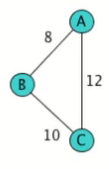
\includegraphics{Kruskal/Grafo3.png}
            \caption{Gráfo de 3 nodos y 3 arcos}
            \label{Grafo3}
        \end{figure}
            
        El archivo que describe la estructura del grafo es:
        \begin{figure}[h!]
            \centering
            \begin{verbatim}
                A{B$8,C$12}
                B{A$8,C$10}
                C{A$12,B$10}
            \end{verbatim}
            \caption{Estructura del grafo \ref{Grafo3} en el archivo}
            \label{ArchivoGrafo3}
        \end{figure} 
        
        Y el árbol mínimo recorrido encontrado fue: \textbf{F\$18=\{ (A,B)  (B,C) \}}
        
        \subsubsection*{Grafo de 4 nodos}
        Grafo muy sencillo de únicamente 4 nodos. Fig\ref{Grafo4} y su estructura en \ref{ArchivoGrafo4}.
        
        \begin{figure}[h!]
            \centering
            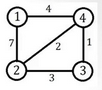
\includegraphics{Kruskal/Grafo4.png}
            \caption{Gráfo de 4 nodos y 5 arcos}
            \label{Grafo4}
        \end{figure}
            
        El archivo que describe la estructura del grafo es:
        \begin{figure}[h!]
            \centering
            \begin{verbatim}
                1{2$7,4$4}
                2{1$7,3$3,4$2}
                3{2$3,4$1}
                4{1$4,2$2,3$1} \end{verbatim}
            \caption{Estructura del grafo \ref{Grafo4} en el archivo}
            \label{ArchivoGrafo4}
        \end{figure} 
        
        Y el árbol mínimo recorrido encontrado fue: \textbf{F\$7=\{ (3,4)  (2,4)  (1,4) \}}
        
        \subsubsection*{Grafo de 5 nodos}
        Grafo de únicamente 5 nodos. Fig\ref{Grafo5} y su estructura en \ref{ArchivoGrafo5}.
        
        \begin{figure}[h!]
            \centering
            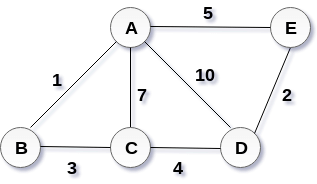
\includegraphics[width=6cm]{Kruskal/Grafo5.png}
            \caption{Gráfo de 5 nodos y 7 arcos}
            \label{Grafo5}
        \end{figure}
            
        El archivo que describe la estructura del grafo es:
        \begin{figure}[h!]
            \centering
            \begin{verbatim}
                A{B$1,C$7,D$10,E$5}
                B{A$1,C$3}
                C{A$7,B$3,D$4}
                D{A$10,C$4,E$2}
                E{A$5,D$2}\end{verbatim}
            \caption{Estructura del grafo \ref{Grafo5} en el archivo}
            \label{ArchivoGrafo5}
        \end{figure} 
        
        Y el árbol mínimo recorrido encontrado fue: \textbf{F\$11=\{ (A,B)  (D,E)  (B,C)  (A,E) \}}
        
        \subsubsection*{Grafo de 6 nodos}
        Grafo de 6 nodos. Fig\ref{Grafo6} y su estructura en \ref{ArchivoGrafo6}.
        
        \begin{figure}[h!]
            \centering
            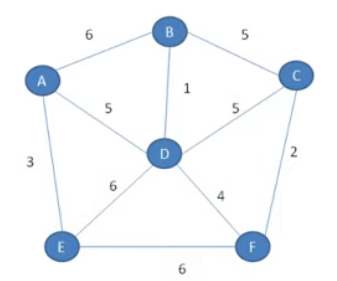
\includegraphics[width=6cm]{Kruskal/Grafo6.png}
            \caption{Gráfo de 6 nodos y 10 arcos}
            \label{Grafo6}
        \end{figure}
            
        El archivo que describe la estructura del grafo es:
        \begin{figure}[h!]
            \centering
            \begin{verbatim}
                A{B$6,D$5,E$3}
                B{A$6,C$5,D$1}
                C{B$5,D$5,F$2}
                D{A$5,B$1,C$5}
                E{A$3,D$6,F$6}
                F{C$2,D$4,E$6}\end{verbatim}
            \caption{Estructura del grafo \ref{Grafo6} en el archivo}
            \label{ArchivoGrafo6}
        \end{figure} 
        
        Y el árbol mínimo recorrido encontrado fue: \textbf{F\$15=\{ (B,D)  (C,F)  (A,E)  (F,D)  (A,D) \}}
        
        \subsubsection*{Grafo de 7 nodos}
        Grafo de 7 nodos. Fig\ref{Grafo7} y su estructura en \ref{ArchivoGrafo7}.
        
        \begin{figure}[h!]
            \centering
            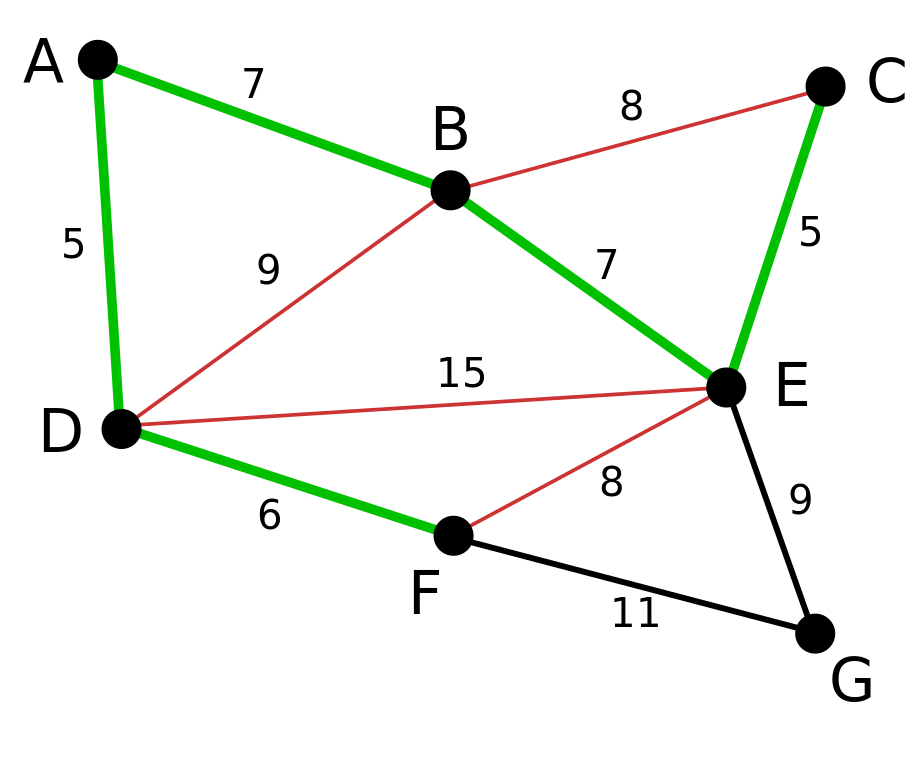
\includegraphics[width=6cm]{Kruskal/Grafo7.png}
            \caption{Gráfo de 7 nodos y 11 arcos}
            \label{Grafo7}
        \end{figure}
            
        El archivo que describe la estructura del grafo es:
        \begin{figure}[h!]
            \centering
            \begin{verbatim}
            A{B$7,D$5}
            B{A$7,C$8,D$9,E$7}
            C{B$8,E$5}
            D{A$5,B$9,E$15,F$6}
            E{B$7,C$5,D$15,F$8,G$9}
            F{D$6,E$8,G$11}
            G{E$9,F$11}\end{verbatim}
            \caption{Estructura del grafo \ref{Grafo7} en el archivo}
            \label{ArchivoGrafo7}
        \end{figure} 
        
        Y el árbol mínimo recorrido encontrado fue: \textbf{F\$41=\{ (C,E)  (A,D)  (D,F)  (B,E)  (E,G)  (B,D) \}}
    
        \newpage
    
        \subsubsection*{Grafo de 8 nodos}
        Grafo de 8 nodos. Fig\ref{Grafo8} y su estructura en \ref{ArchivoGrafo8}.
        
        \begin{figure}[h!]
            \centering
            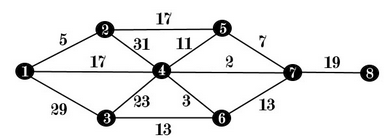
\includegraphics[width=6cm]{Kruskal/Grafo8.png}
            \caption{Gráfo de 8 nodos y 13 arcos}
            \label{Grafo8}
        \end{figure}
            
        El archivo que describe la estructura del grafo es:
        \begin{figure}[h!]
            \centering
            \begin{verbatim}
            1{2$5,3$29,4$17}
            2{1$5,4$31,5$17}
            3{1$29,4$23,6$13}
            4{1$17,2$31,3$23,5$11,6$3,7$2}
            5{2$17,4$11,7$7}
            6{3$13,4$3,7$13}
            7{4$2,5$7,6$13,8$19}
            8{7$19}\end{verbatim}
            \caption{Estructura del grafo \ref{Grafo8} en el archivo}
            \label{ArchivoGrafo8}
        \end{figure} 
        
        Y el árbol mínimo recorrido encontrado fue: \textbf{F\$64=\{ (4,7)  (4,6)  (1,2)  (5,7)  (3,6)  (2,5)  (1,4) \}}

    \newpage

        \subsubsection*{Grafo de 9 nodos}
        Grafo de 9 nodos. Fig\ref{Grafo9} y su estructura en \ref{ArchivoGrafo9}.
        
        \begin{figure}[h!]
            \centering
            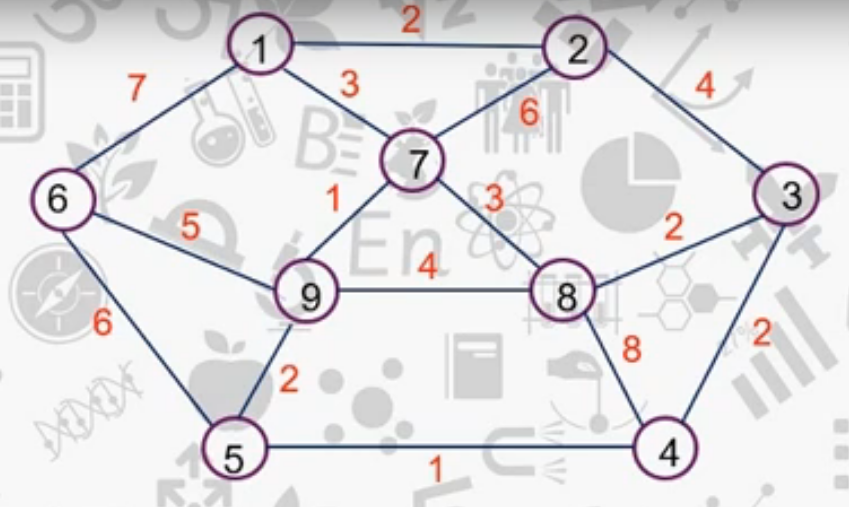
\includegraphics[width=6cm]{Kruskal/Grafo9.png}
            \caption{Gráfo de 9 nodos y 15 arcos}
            \label{Grafo9}
        \end{figure}
            
        El archivo que describe la estructura del grafo es:
        \begin{figure}[h!]
            \centering
            \begin{verbatim}
            1{2$2,7$3,6$7}
            2{1$2,7$6,3$4}
            3{2$4,8$2,4$2}
            4{3$2,8$8,5$1}
            5{4$1,9$2,6$6}
            6{5$6,9$5,1$7}
            7{1$3,2$6,8$3,9$1}
            8{3$2,4$8,9$4,7$3}
            9{7$1,8$4,5$2,6$5}\end{verbatim}
            \caption{Estructura del grafo \ref{Grafo9} en el archivo}
            \label{ArchivoGrafo9}
        \end{figure} 
        
        Y el árbol mínimo recorrido encontrado fue: \textbf{F\$18=\{ (7,9)  (4,5)  (5,9)  (3,4)  (3,8)  (1,2)  (1,7)  (6,9) \}}
    
    \newpage
    
        \subsubsection*{Grafo de 10 nodos}
        Grafo de 10 nodos. Fig\ref{Grafo10} y su estructura en \ref{ArchivoGrafo10}.
        
        \begin{figure}[h!]
            \centering
            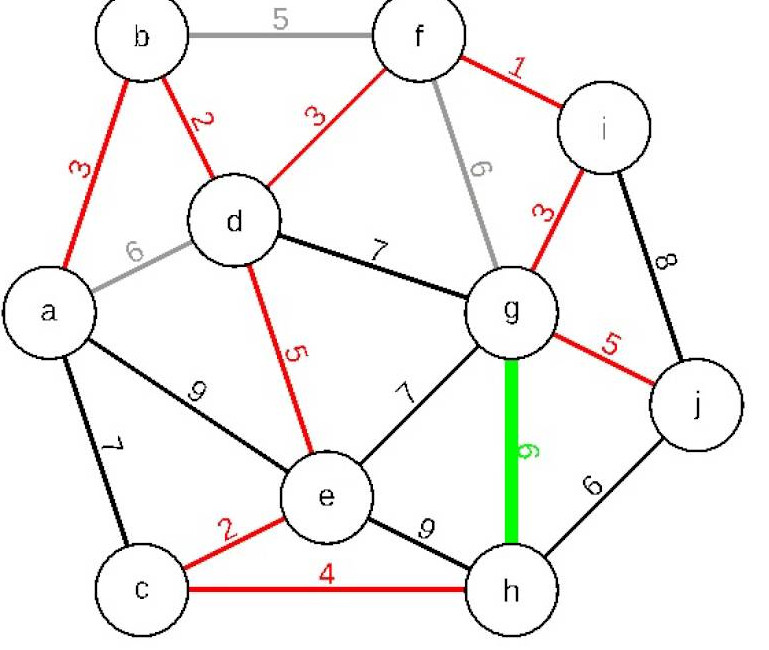
\includegraphics[width=6cm]{Kruskal/Grafo10.jpeg}
            \caption{Gráfo de 10 nodos y 15 arcos}
            \label{Grafo10}
        \end{figure}
            
        El archivo que describe la estructura del grafo es:
        \begin{figure}[h!]
            \centering
            \begin{verbatim}
            a{b$3,d$6,e$9,c$7}
            b{a$3,d$2,f$5}
            c{a$7,e$2,h$4}
            d{a$6,b$2,e$5,f$3,g$7}
            e{a$9,c$2,d$5,g$7,h$9}
            f{b$5,d$3,g$6,i$1}
            g{d$7,e$7,f$6,h$6,i$3,j$5}
            h{c$4,e$9,g$6,j$6}
            i{f$1,g$3,j$8}
            j{g$5,h$6,i$8}\end{verbatim}
            \caption{Estructura del grafo \ref{Grafo10} en el archivo}
            \label{ArchivoGrafo10}
        \end{figure} 
        
        Y el árbol mínimo recorrido encontrado fue: \textbf{F\$28=\{ (f,i)  (c,e)  (b,d)  (g,i)  (d,f)  (a,b)  (c,h)  (g,j)  (b,f) \}}
        
        \newpage
        
        \subsubsection{Propuesta de complejidad}
        A partir de estos 8 archivos ingresados y evaluados por el programa, la gráfica en la figura \ref{GraficaKruskal} muestra el resultado de la comparación del número de nodos o aristas del grafo ingresado, contra el número de operaciones realizadas para cada archivo:
        \begin{figure}[h!]
            \centering
            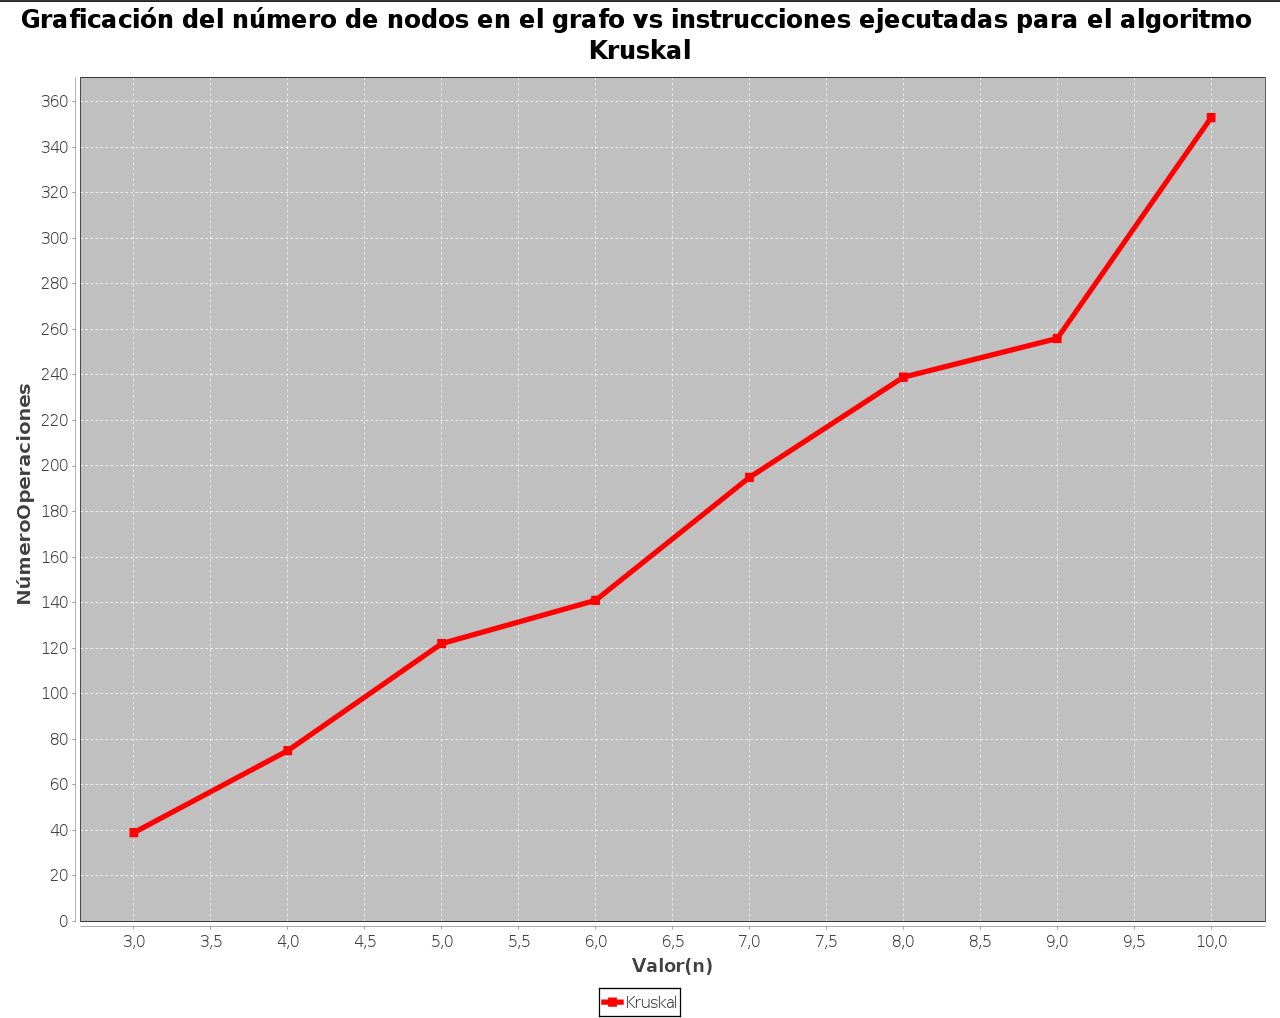
\includegraphics[width=16cm]{Kruskal/GraficaKruskal.png}
            \caption{Gráfica generada a partir de la evaluación de los archivos con los grafos descritos\\ En el eje de las abcisas se encuentra el número de nodos del grafo y en el de las ordenadas el número de operaciones realizadas}
            \label{GraficaKruskal}
        \end{figure}
        Y los puntos que genera esta gráfica son \ref{PuntosKruskal}:
        \begin{figure}[h!]
            \centering
            \begin{tabular}{c c}
                P1( 3 ,39 ) & P5( 7 ,195 ) \\
                P2( 4 ,75 ) & P6( 8 ,239 )\\
                P3( 5 ,122 ) & P7( 9 ,256 )\\
                P4( 6 ,141 ) & P8( 10 ,353 )\\
            \end{tabular}
            \caption{Puntos obtenidos de la evaluacion de los 8 grafos especificados anteriormente}
            \label{PuntosKruskal}
        \end{figure}
        
        Y es con estos datos obtenidos que se propone la complejidad para este algoritmo. En la figura \ref{GraficaComplejidadKruskal} se muestran los puntos obtenidos y 2 ecuaciones que acotan a estos mismos. Es evidente desde la figura \ref{GraficaKruskal} que su cota superior no podría ser lineal pues el crecimiento que experimenta en el eje de las ordenadas es muy veloz en comparación con una complejidad lineal.\\
        
        \begin{figure}[h!]
            \centering
            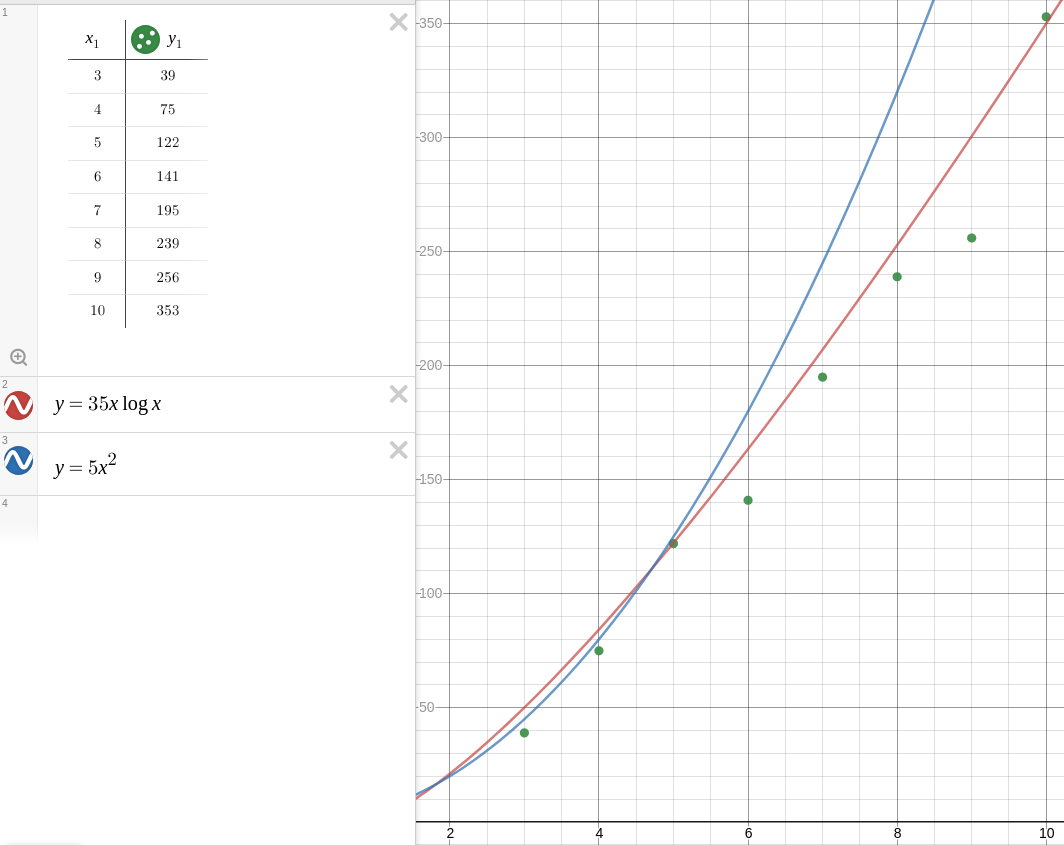
\includegraphics[width=19cm]{Kruskal/GraficaComplejidadKruskal.png}
            \caption{Gráfica de la proposición para la complejidad para el algoritmo de Kruskal\\ Los puntos verdes corresponden a los puntos obtenidos de la evaluación de los grafos \\ La curva de color rojo corresponde a la cota de orden \textit{n logn}\\ La curva de color azul corresponde a la cota de orden $n^2$}
            \label{fig:my_label}
        \end{figure}
        
        Por esta razón se propone hacer una comparación de las 2 cotas siguientes superiores, la cota \textit{nlogn} y $n^2$.\\
        
        Mediante la asignación arbitraria de valores constantes que multiplican a los términos, observamos claramente que una cota del orden \textit{nlogn}, se ajusta de forma más justa y describiendo un comportamiento parecido al de los puntos.\\
        
        Mientras que la cota cuadrática en un principio parece acotar de forma más justa a los primeros 3 puntos, su crecimiento será muy superior con los datos obtenidos posteriores.\\
        
        De tal manera que se afirma que para el algoritmo de Kruskal que permite encontrar un árbol mínimo recubridor en un grafo conexo no dirigido y ponderado será:
        \begin{equation*}
            \text{\textbf{kruskal(n)}}\in\text{\textbf{O(n log n)}}
        \end{equation*}

\subsection*{Investigación complejidad}

    Los elementos escenciales para el funcionamiento del algoritmo, y por consiguiente los que nos darán el tiempo de ejecución, serán en general el grafo, pero siendo más especificos, los elementos que componen al arbol. Las aristas(\textbf{a}) y los vértices(\textbf{v}), que ya se especificó antes se encuentran ponderados mediante un costo, son los 2 elementos principales que intervienen en la complejidad del algoritmo.\\
    
    Se considera que para el algoritmo de Kruskal la complejidad será a lo más \textbf{O(a log a)}, siendo equivalente la cota \textbf{O(a log n)}, cuando los datos se encuentran almacenados mediante estructuras simples.\\
    
    La razón por la que estas 2 cotas son equivalentes se debe a:
    \begin{itemize}
        \item Las aristas serán a los más $v^2$, y el $logv^2 = 2logv$ que puede calcularse mediante diversos métodos, pero otorga una complejidad de \textbf{O(log v)}
        \item Se ignoran los vértices aislados, esto debido que forman su propia componente del árbol de expansión mínimo, los vertices son menores o iguales a el doble de las aristas $v\leq 2a$, resultando entonces que el logn es \textbf{O(loga)}
    \end{itemize}
    
    Para poder conseguir esta complejidad es primordial ordenar las aristas en función del peso, mediante un algoritmo con complejidad \textit{O(a log a)}, como lo es \textit{Comparison sort}. Esta ordenación permite que la eliminación de una arista con peso mínimo pueda ejecutarse en un tiempo constante.\\
    
    Ahora, dado que es necesario el control de los vértices para identificar cuales de estos están en que componentes, se utiliza una estructura de datos sobre conjuntos disjuntos. La complejidad del ordenamiento de este será \textit{O(a)} operaciones, esto se debe a 2 operaciones de búsqueda por arista, y una posible unión de conjuntos.\\
    
    Finalmente se considera que inclusive con una estructura de conjuntos disjuntos simples con uniones poir rangos, es capaz de ejecutar las operaciones mencionadas en un tiempo \textbf{O(a log v)}, se considera que el orden de este algoritmo es:
    \begin{equation*}
        \text{\textbf{O(a log a) = O(a log v)}}
    \end{equation*}
    
    Este algoritmo permite además encontrar soluciones para estructuras de conjuntos disjuntos complejos, tales como los bosques, es posible acotar los tiempos de ejecución en \textbf{O(a $\alpha$(v))}, de donde $\alpha$ es la inversa de la \textit{Función de Ackermann}.\\
    
    La función de \textit{Ackermann}, es un función matemática recursiva que fue encontrada en el año de 1926 por el matemático alemán Willhelm Ackermann. Que tienen cono particularidad, un crecimiento extremadamente rápido, lo que consecuentemente las volvería un recurso interesante para la ciencia computacional teórica y la teoría de computabilidad.\\
    
    Es precisamente por esta característica, que el valor de su inversa tendrá el comportamiento contrario, un crecimiento sumamente lento, dotando de una complejidad aún muy controlada inclusive cuando se trabaja con estructuras complejas para el algoritmo de Kruskal.